\documentclass[conference]{IEEEtran}
\usepackage{enumitem}
\usepackage[document]{ragged2e}
\usepackage{blindtext}
\usepackage{graphicx}
\usepackage{float}
\usepackage{amsmath}
%\usepackage{natbib}
\usepackage{cite}

\graphicspath{ {./}{./images/} }

\title{Joint Radar Communication System using OFDM}

\author{

\IEEEauthorblockN{Owen Sowatzke}
\IEEEauthorblockA{\textit{Electrical Engineering Department} \\
\textit{University of Arizona}\\
Tucson, USA \\
osowatzke@arizona.edu}

\and
\IEEEauthorblockN{Iman Miraki}
\IEEEauthorblockA{\textit{Electrical Engineering Department} \\
\textit{University of Arizona}\\
Tucson, USA \\
imanmiraki@arizona.edu}}

\begin{document}
	\raggedbottom
	\maketitle
\section {Introduction}
     Vehicle-to-Vehicle (V2V) networks seek to enhance road safety and reduce traffic congestion by sharing road and traffic information between vehicles in real time. To avoid delays associated with third party networks, vehicle-to-vehicle communication systems need dedicated bandwidth. Instead of wasting additional spectrum resources, joint radar communication (JRC) systems attempt to integrate radar and communication systems. This results in reduced bandwidth usage and reduced power consumption while eliminating the need for additional hardware.
     
     In this paper, we design a JRC system, which uses OFDM for communication and zero-forcing to generate a range response from the OFDM returns. Next, we examine the performance of this system and compare it to standalone radar and standalone OFDM implementations.
        
  \section {Radar}
   \subsection {Background}
   
In this section, we provide background on frequency-modulated continuous wave (FMCW) radar, which is used in many automotive applications. FMCW radar continuously transmits a signal whose frequency varies linearly over time (chirp). It measures the time delay between the transmitted and the reflected signals (echoes) to determine the distance of reflecting objects. It can also determine the relative velocity of these objects, by measuring frequency shifts caused by the doppler effect.

	\begin{figure}[H]
    		\centering
    		\fbox{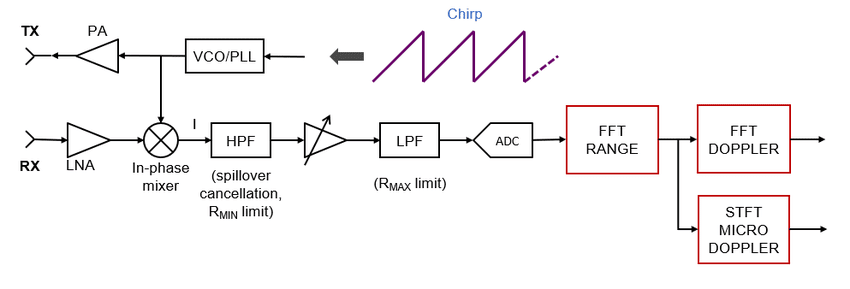
\includegraphics[width=0.9\linewidth]{FMCW Blockdiagram}}
    		\caption{Typical FMCW blockdiagram \cite{9613183}}
    		\label{fig::fmcw_radar}
	\end{figure}
	
 The block diagram shown in Figure \ref{fig::fmcw_radar} depicts the signal processing chain of a typical FMCW radar system. The transmitter generates a frequency-modulated chirp signal of the following form:
 
 	\begin{equation}
 		x(t) = e^{j\pi{\beta}t^2/\tau}
 		\label{eq::chirp}
 	\end{equation}
 	
 	where $\beta$ is the chirp bandwidth and $\tau$ is the chirp duration.
 	
	It transmits this signal out of the antenna towards objects of interest. The receiver receives reflections from each of these objects, which are passed through a low noise amplifier. For each return, the received signal will be a chirp waveform with a frequency offset as illustrated below.
	
	\begin{equation}
		r(t) = e^{j\pi{\beta}(t - t_0)^2/\tau} = e^{j\pi{\beta}t^2/\tau}e^{-j2\pi({\beta}t_0/\tau)t}e^{j\pi{\beta}t_0^2/\tau}
		\label{eq::delayed_chirp}
	\end{equation}
	
	We can mix the received signal with the transmitted signal to create a tone for each return. The frequency of this tone will be proportional to its delay.
	
	\begin{equation}
		f = \frac{{\beta}t_0}{\tau} \Rightarrow t_0 = \frac{{\tau}f}{\beta}
	\end{equation}
	
	The delay of this return is then related to the range of the reflecting object as follows:
	
	\begin{equation}
		R = \frac{ct_0}{2}
	\end{equation}
	
	The relationship between the transmitted and received chirps signals is illustrated below:
	
	\begin{figure}[H]
    		\centering
    		\fbox{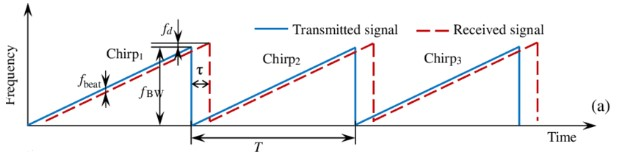
\includegraphics[width=0.8\linewidth]{FMCW Freq-Time graph}}
    		\caption{Typical FMCW transmitted and Received signal, Time vs Frequency graph \cite{Long2019AssistingTV}}
    		\label{fig::fmcw_spectrogram}
	\end{figure}
	
	Note that the chirp bandwidth $\beta$ is inversely proportional to the range resolution ${\Delta}R$.
	
	\begin{equation}
		{\Delta}R = \frac{c}{2\beta}
	\end{equation}
	
	Because fine range resolution is desired, $\beta$ is typically very large (on the order of 150MHz-500MHz). This would typically require very high sample rates. However, one of the benefits of an FMCW radar is that the ADC input is tones instead of a full bandwidth signal. Thus, we only need to sample at a rate high enough to capture returns at the largest range of interest. For an automotive radar, this may only be on the order of 100-200 m, which can significantly reduce the sample rates and in turn reduce the radar's cost.
	
	After low-pass filtering and sampling the signal, Figure \ref{fig::fmcw_radar} illustrates the next step in the signal processing (a fast-time FFT). This FFT detects the frequency of each tone, which is proportional to the object's distance.
	
	The target's relative velocity results in a doppler shift:
	
	\begin{equation}
		f_D = \frac{2v}{\lambda}
	\end{equation}
	
	Note that this doppler shift is twice what is for a communication system, due to the reflection's two-way path. The phase change due to the doppler shift is small during a single chirp, so we instead measure it over multiple chirps (pulses). This is done by taking an FFT across pulses as shown in Figure \ref{fig::fmcw_radar}.
	
	The rate at which chirps (pulses) are repeated is denoted as the PRF. The PRF limits the radar's unambiguous velocity $v_{ua}$ and unambiguous range $R_{ua}$. If a return exceeds these limits, it will alias to another range or velocity.
	
	\begin{equation}
		v_{ua} = \frac{\lambda\cdot\text{PRF}}{4}
	\end{equation}
	
	\begin{equation}
		R_{ua} = \frac{c}{2\cdot\text{PRF}}
	\end{equation}
	
The main purpos of the radar, estimating velocity and range of the target, is acuratly achievable with FMCW signlas. The mathotalegy can be simply comprehented by the graph below. The range FFT provides the beat frequency to calculate the target distance and doppler FFT provides the frequncy delta between trnasmitted and received signal to calculate the target velocity. 
	

Some of Radar's perform metrics of interest that we are going to analize in this paper include but are not limited to:

\begin{itemize}
\item Received SNR
\item Maximum Resolvable Range
\item Range Resolution
\item Doppler Tolerance
\item Peak Sidelobe Level (PSL)
\end{itemize}

	Range (targer distance) can be calculated from equation \ref{eq::range_calculation}. %simple formula below:
	
	\begin{equation}
		R = \frac{c_0|{\Delta}t|}{2} = \frac{c_0|{\Delta}f|}{2\left(\frac{df}{dt}\right)}
		\label{eq::range_calculation}
	\end{equation}
	
	\begin{itemize}
	\item Co = speed of light = 3·108 m/s
	\item \(\Delta \)t = delay time [s]
	\item \(\Delta \)f = measured frequency difference [Hz]
	\item R = distance between antenna and the reflecting object (ground) [m]
	\item df/dt = frequency shift per unit of time
	\end{itemize}

Other critical parameters to consider for a radar performance are range resolution and Doppler/range ambiguity. 
Maximum unambiguous range is calculated from formula below:

	\begin{equation}
		R_{max} = \frac{c_0}{2.PRF}
		\label{eq:: range ambiguity_calculation}
	\end{equation}

Maximum unambiguous Doppler velocity is calculated from formula below:

\begin{equation}
		V_{max} = \frac{PRF.\lambda}{4}
		\label{eq:: Doppler ambiguity_calculation}
	\end{equation}
  
  Where PRF is Pulse Repetition Frequency (number of pulse per second).

In the interest of comparing FMCW with JRC methode, we outline few advantages of FMCW in radar.
	\begin{itemize}
		\item High range resolution
		\item Continuous operation
		\item Simultaneous range and velocity measurement
		\item Simple hardware
		\item Low power consumption
	\end{itemize}
	



	\subsection {Simulation and Performance}

In this section, we evaluate the performance of an FMCW radar written in MATLAB, and configured with the following set of parameters:

	\begin{center}
	\begin{tabular}{|c|c|}
		\hline
		Parameter & Value \\
		\hline
		Carrier Frequency & 77 GHz \\
		\hline
		Sample Rate & 300 MHz \\
		\hline
		PRF & 200 kHz \\
		\hline
		Number of Pulses & 256 \\
		\hline	
	\end{tabular}
	\end{center}
	
	Metrics of interest include the received SNR, unambiguous range, unambiguous velocity, range resolution, doppler tolerance, and peak sidelobe level (PSL).

	\begin{itemize}
		\item Received SNR
		\item Unambiguous Range
		\item Range Resolution
		\item Doppler Tolerance
		\item Peak Sidelobe Level (PSL)
	\end{itemize}

The radar has been configured with the following set of parameters:

 as the results of the FMCW radar simulation that was coded with Matlab. The code written programaticaly to allow us easily change the parameters to match the JRC wave and channel properties. This is necessery to have the comprehensive and fair comparison between FMCW and JRC performance. 
The results below are extracted from the FMCW  radar simulation with parameter below:

	
	
	\begin{itemize}
	\item Carrier Frequency:	77 GHz
	\item Sampling Rate:		200 MHz
	\item PRF:				500 KHz
	\item Code Length:		127
	\item SNR:				20 dB
	\end{itemize}
	
Simulation contains of generating the chirp signal for transmission, simulatin gthe received signal with target delays, Doppler shifts and noise. Windowin gis applied in both steps to reduce spectral leakage. The produced results are  FFT oerations in both fast and slow time. It supports multiple targets and includes configurable parameters like bandwidth, sample rate, and windowing functions. Graph below is the result of fast-time FFT displaying the target range.

	\begin{figure}[H]
	    		\centering
	    		\fbox{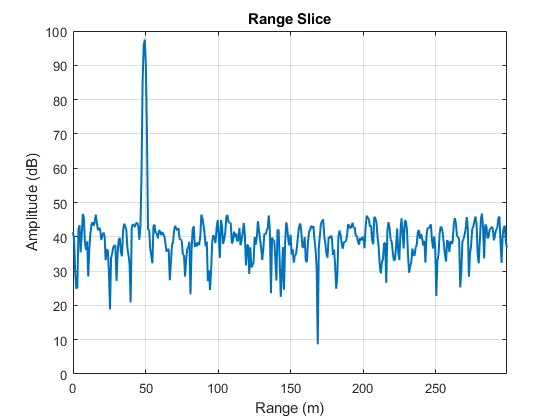
\includegraphics[width=0.8\linewidth]{FMCW_Range Slice}}
	    		\caption{FMCW range slice}
		\end{figure}

Graph below is the result of slow-time FFT, displaying the target velocity by analizing the phase change over multiple chirps. 

	\begin{figure}[H]
	    		\centering
	    		\fbox{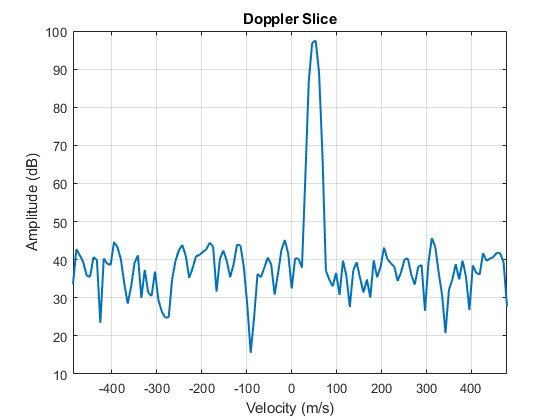
\includegraphics[width=0.8\linewidth]{FMCW_Doppler Slice}}
	    		\caption{FMCW Doppler slice}
		\end{figure}
	
Graph below is the result of mixing both Range and Doppler FFT. The Range-Doppler map's X-axis is a Doppler bins (relative velocity) and Y-axis is a range bins (distance). Bright spots indicate targets and their corresponding tange and velocity.
	\begin{figure}[H]
	    		\centering
	    		\fbox{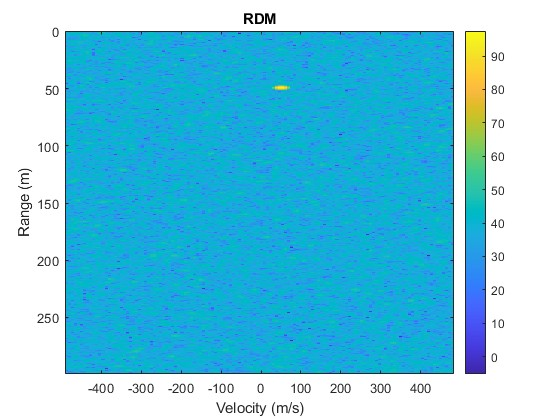
\includegraphics[width=0.8\linewidth]{FMCW_RDM}}
	    		\caption{FMCW Range Doppler Map}
		\end{figure}
		
		
     \section {Communication (OFDM)}
     
	 \subsection {Background}
 
 
            In this section we skim through OFDM communicaiton protocol. Since the objective of this paper is V2V JRC our focus is on IEEE 802.11 P standard. In this section we familiarize ourself with the functionality, key features, some 802.11 P standard specificaitons and advantages of this communication topology.\par
    \textbf{  802.11 P} is specifically designed for wireless access in vehicular environments (WAVE) and is widely used for V2V applications within the automotive industry.
      
      \begin{itemize}
      \item Frequency Band:		5.850 GHz to 5.925 GHz (DSRC Band)
	\item Channel Bandwidth:	10 MHz
	\item Modulation:		BPSK, QPSK, 16-QAM
	\item Maximum Data Rate:	27 Mbps (Theoretical)
	\item Range: 			Up to 1 km (ideal conditions)
	\item Vehicle Speed :                Up to 200 km/h
	\item Security:			WPA2, Authentication, Message Integrity
	\item Applications:		Collision avoidance, traffic management, V2X
	\end{itemize}
	
 \textbf{ Orthogonal Frequency Division Multiplexing (OFDM)} is widely used in Vehicle-to-Vehicle (V2V) communication systems for several reasons, including inherent characteristics that provide efficient data transmission in dynamic, high-speed environments.

Block diagram below is a typical OFDM process from input bit steam, modulation, through the channel, DFT, demodulation and output bit steam. 

		\begin{figure}[H]
	    		\centering
	    		\fbox{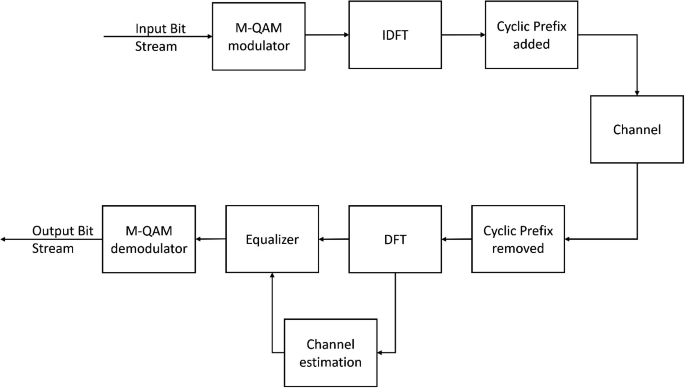
\includegraphics[width=0.9\linewidth]{OFDM Block diagram}}
	    		\caption{OFDM block diagram}
		\end{figure}
      
      The graph below illustrat a typical OFDM fram (64-subcarrier example)
      
      	\begin{itemize}
      	\item Guard Band (Zero Subcarriers): Subcarriers 0–5 and 59–63
	\item Data Subcarriers: Subcarriers 6–28 and 37–58
	\item Pilot Subcarriers: Subcarriers 7, 21, 43, 57
	\item DC Subcarrier (Zero): Subcarrier 32
	\end{itemize}

	\begin{figure}[H]
	    		\centering
	    		\fbox{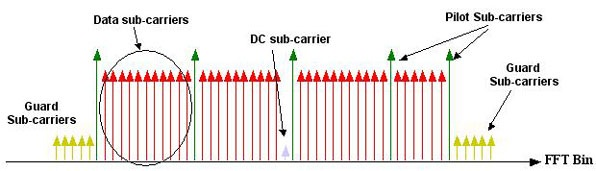
\includegraphics[width=0.9\linewidth]{OFDM subcarriers}}
	    		\caption{OFDM subcarriers}
		\end{figure}
		
Some of OFDM's perform metrics of interest that we are going to analize in this paper include but are not limited to:

\begin{itemize}
\item Received SNR
\item Bit Error Rate (BER)
\item Channel Capacity
\end{itemize}

One channel's property needs to be analysed and compared is the channel capacity. We use the simple fromula below (Shannon-Hartley theorem) to calculate the channel capacity. 
Where Bk is the bandwidth of the k-th subcarrier, Pk, transmit power, Hk, frequency response magnitude and Nk is a noise power.   
%Where H (m, n) , Hmn is the channel frequency response of the n symbol on the m sub carrier. 
	
		%\begin{equation}
		%	    		C_{m,n} = \text{log}_2\left(1 + \text{SNR}|H(m,n)|^2\right)
	    	%	\label{eq:ofdm_capacity}
		%\end{equation}

			\begin{equation}
			C_{k} = B_{k}.\text{log}_2\left(1 +\frac{ \text P_{k}.|H_{k}|^2}{N_{k}}\right)
	    		\label{eq:ofdm_capacity}
	    		\end{equation}

\subsection {Simulation and Performance}
      
      We have developed comprehensive MATLAB code to evaluate and plot the Bit Error Rate (BER) versus SNR across various channel conditions.. Evaluating diverse channel characteristics is key to achieving a comprehensive and unbiased analysis in our study. The summary implemntation of a complete OFDM simulation model parameters and results for AWGN, Rayleight Fading and perfect channel provided below. 
      
\begin{itemize}
\item 64 Subcarriers, 48 Data carriers, 10 K Symbols adn 16 Cyclic-prefix
\item 4th order QAM modulation and 10 MHz Sample rate
\item Pilots are inserted at standard intervals and zero carriers are placed at the edges of the spectrum.
\item The IFFT converts the frequency domain symbols to the time domain. 
\item A Hamming window is applied to each OFDM symbol to reduce spectral leakage. 
\item A cyclic prefix is added to the windowed OFDM symbols to mitigate ISI. 
\item An AWGN channel is used to transmit the flattened signal to the receiver.\par
\item The receiver removes the cyclic prefix. 
\item The data sub-carriers are extracted and demodulated from FFT, results in frequency domain. 
\item The received bits are compared to the transmitted bits to calculate the BER vs SNR values. 
\end{itemize}
The power spectral density of trasmitted OfDM signal shown in the graph below. The flat region conrresponds to the active subcarriers of the OFDM signal (each subcarrier carries equal power and spans the same bandwidth). There is a dip null in the center correspoinding to the DC (zero frequency) subcarrier which used to avoid interference. The dips at the edges are the guard bands to rduce spectral leakage and interference with adjacent channels.

	\begin{figure}[H]
    		\centering
    		\fbox{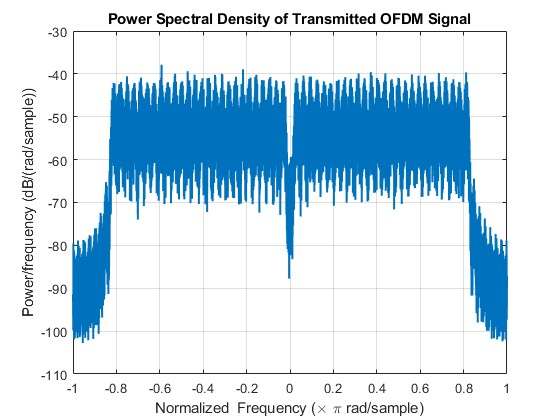
\includegraphics[width=0.8\linewidth]{OFDM Power spectral density}}
    		\caption{OFDM Power Spectral Density}
	\end{figure}

  The graph below is a constellation coresponding to 4th order QAM with AWGN channel propery.  The points are tightly packed around the ideal constellation locations, indicating that noise has minimal impact on the received signal (high SNR conditions).This diagram demonstrates that the system performs well under high SNR conditions, maintaining accurate symbol transmission and reception.
    
    
     \begin{figure}[H]
		\centering
    		\fbox{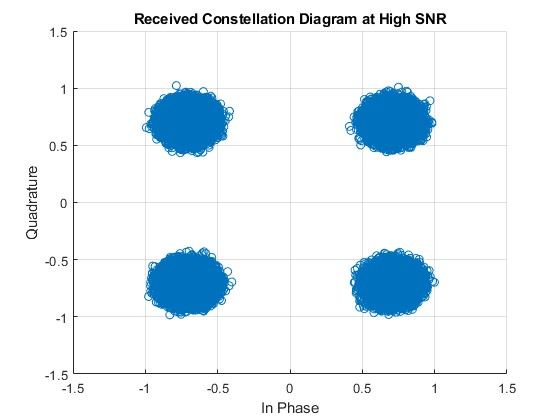
\includegraphics[width=0.8\linewidth]{OFDM AWGN Constellation}}
    		\caption{OFDM Constellation Diagram  (AWGN) }
  	  \end{figure}
    
    The BER decreases exponentially as the SNR increases, which is typical for digital communication systems. The close alignment of the measured and reference curves validates the simulation accuracy and ensures the OFDM system is working as intended. The system shows robust performance at higher SNR values, achieving nearly error-free communication. This analysis is crucial for validating the system and ensuring its effectiveness in real-world applications.
    
    
         \begin{figure}[H]
		\centering
    		\fbox{\includegraphics[width=0.8\linewidth]{OFDM AWGN BER vs SNR}}
    		\caption{OFDM BER vs. SNR (AWGN) }
  	  \end{figure}
    

  The results below are from the same signal charactristics transmitted through Rayleigh fading channel. The points are tightly clustered around the ideal constellation positions (caused by delay fading) that implying effective channel conditions and robust equalization process. The constellation diagram results indicates that the system operates in a highl SNR environment where noise has minimal impact. 

	\begin{figure}[H]
		\centering
    		\fbox{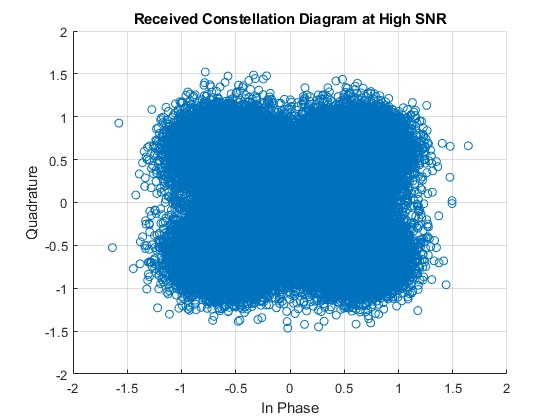
\includegraphics[width=0.8\linewidth]{OFDM Constellation Diagram}}
    		\caption{OFDM Constellation Diagram  (Rayleigh)}
  	  \end{figure}

The plot below represents the Bit Error Rate (BER) vs. Signal-to-Noise Ratio (SNR) performance of an OFDM system. It compares the measured BER from the simulation against the theoretical (reference) BER for the given modulation scheme and channel model. Both curves show a monotonic decrease in BER with increasing SNR, which is expected as higher SNR improves the signal quality and reduces errors. Around 6-10 dB, the curve begins to drop sharply, indicating the SNR threshold beyond which the system transitions from error-prone to error-free performance. This plot confirms that the OFDM system performs reliably under high SNR and aligns closely with theoretical predictions.
    
    \begin{figure}[H]
		\centering
    		\fbox{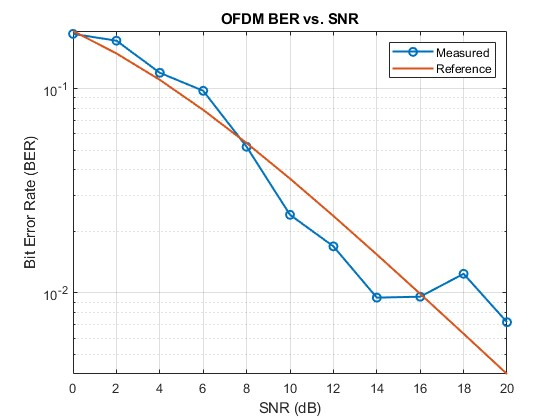
\includegraphics[width=0.8\linewidth]{OFDM BER vs SNR}}
    		\caption{OFDM BER vs. SNR}
  	  \end{figure}    
  	  
  	  For the given parameter, B total=10 MHz, N subcarriers=64, N data=48, P total =1 W (assumed for simplicity) and No=1 nW/Hz, the total channels capacity for given OFDM  with AWGN is around 99.74 Mbps. \par
  	 It is important to highlight the cyclic prefix reduces the effective data rate, which slightly decreases the channel capacity. Adjust for this overhead if needed.
 
  	  
    
    \section {JRC}
		 \subsection {Background}
		 
 The convergence of radar and communication systems, often referred to as joint radar-communication (JRC), has emerged due to several technological and practical motivations. Some of the primary reasons why radar and communication systems are being integrated listed below :
 
 \begin{itemize}
 \item Spectrum Sharing adn Efficiency (coexisting within the same frequency band)
\item Shared Hardware
\item Autonomous Vehicles
\item Energy Efficiency		 
\end{itemize}		 
		 
The orthogonality or low correlation of the frequency domain allows the two subsystems not to interfere with each other. The disadvantage is that the spectrumutilization of the system is low and energy sharing is difficult to achieve. Other crutial disadvantage we need to overcome is OFDM signals are sensitive to the Doppler shift and multipath effects, which leads to a loss of subcarrier orthogonality and intersymbol interference (ISI) \cite{9992221}.

\subsection {Simulation and Performance}
      


	\bibliographystyle {IEEEtran}
	\bibliography {References}
	
	%\nocite{yang_subcarrier_multiplexing}
	%\bibliography{sources}{}
   % \bibliographystyle{ieeetr}
  
\end{document}

